% Created by tikzDevice version 0.12.6 on 2024-02-27 08:55:26
% !TEX encoding = UTF-8 Unicode
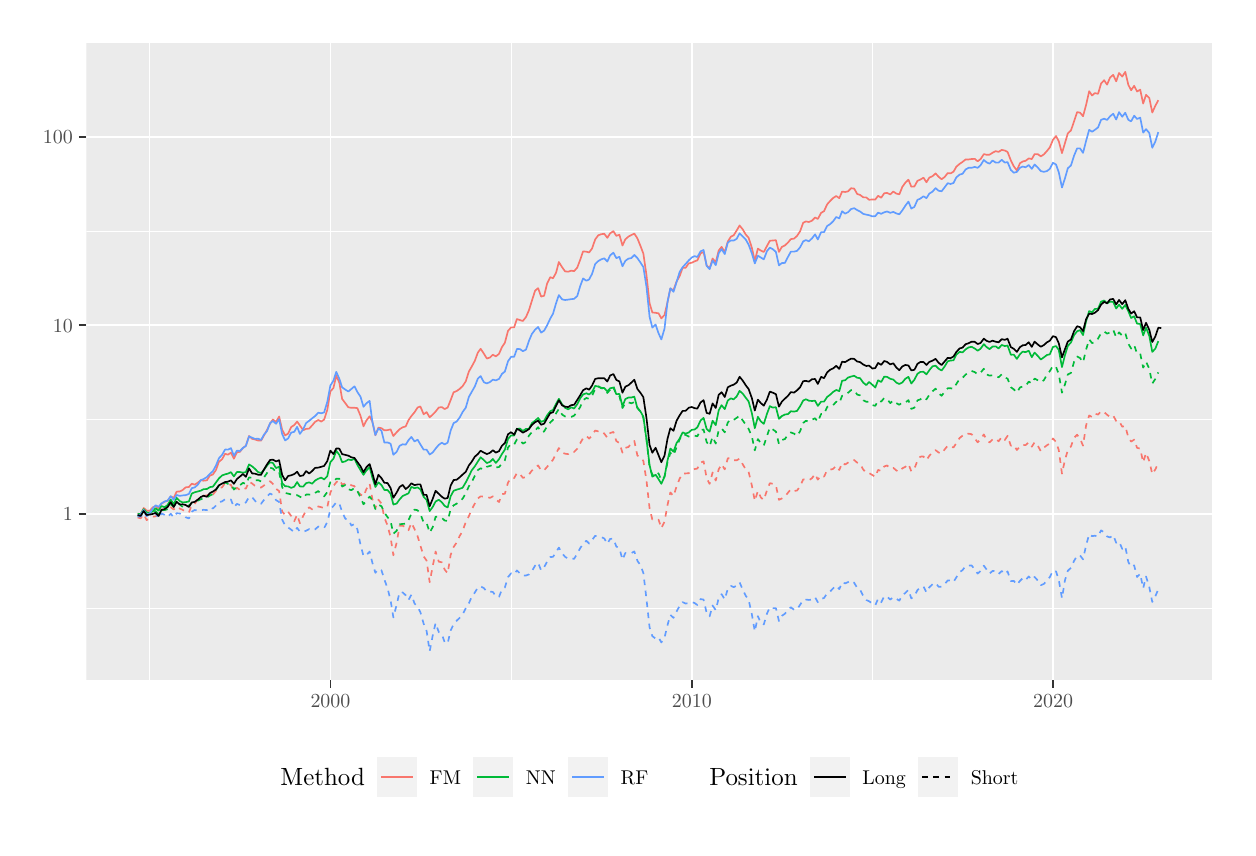
\begin{tikzpicture}[x=1pt,y=1pt]
\definecolor{fillColor}{RGB}{255,255,255}
\path[use as bounding box,fill=fillColor,fill opacity=0.00] (0,0) rectangle (433.62,289.08);
\begin{scope}
\path[clip] (  0.00,  0.00) rectangle (433.62,289.08);
\definecolor{drawColor}{RGB}{255,255,255}
\definecolor{fillColor}{RGB}{255,255,255}

\path[draw=drawColor,line width= 0.6pt,line join=round,line cap=round,fill=fillColor] (  0.00,  0.00) rectangle (433.62,289.08);
\end{scope}
\begin{scope}
\path[clip] ( 21.25, 53.26) rectangle (428.12,283.58);
\definecolor{fillColor}{gray}{0.92}

\path[fill=fillColor] ( 21.25, 53.26) rectangle (428.12,283.58);
\definecolor{drawColor}{RGB}{255,255,255}

\path[draw=drawColor,line width= 0.3pt,line join=round] ( 21.25, 79.30) --
	(428.12, 79.30);

\path[draw=drawColor,line width= 0.3pt,line join=round] ( 21.25,147.45) --
	(428.12,147.45);

\path[draw=drawColor,line width= 0.3pt,line join=round] ( 21.25,215.61) --
	(428.12,215.61);

\path[draw=drawColor,line width= 0.3pt,line join=round] ( 44.12, 53.26) --
	( 44.12,283.58);

\path[draw=drawColor,line width= 0.3pt,line join=round] (174.69, 53.26) --
	(174.69,283.58);

\path[draw=drawColor,line width= 0.3pt,line join=round] (305.25, 53.26) --
	(305.25,283.58);

\path[draw=drawColor,line width= 0.6pt,line join=round] ( 21.25,113.37) --
	(428.12,113.37);

\path[draw=drawColor,line width= 0.6pt,line join=round] ( 21.25,181.53) --
	(428.12,181.53);

\path[draw=drawColor,line width= 0.6pt,line join=round] ( 21.25,249.69) --
	(428.12,249.69);

\path[draw=drawColor,line width= 0.6pt,line join=round] (109.41, 53.26) --
	(109.41,283.58);

\path[draw=drawColor,line width= 0.6pt,line join=round] (239.98, 53.26) --
	(239.98,283.58);

\path[draw=drawColor,line width= 0.6pt,line join=round] (370.52, 53.26) --
	(370.52,283.58);
\definecolor{drawColor}{RGB}{248,118,109}

\path[draw=drawColor,line width= 0.6pt,line join=round] ( 39.74,113.51) --
	( 40.81,113.25) --
	( 41.92,115.51) --
	( 42.99,114.60) --
	( 44.07,114.46) --
	( 45.21,115.77) --
	( 46.21,116.15) --
	( 47.32,115.36) --
	( 48.32,117.05) --
	( 49.50,117.81) --
	( 50.57,118.10) --
	( 51.68,119.70) --
	( 52.79,119.18) --
	( 53.82,121.42) --
	( 54.97,121.49) --
	( 56.04,122.04) --
	( 57.08,122.97) --
	( 58.26,123.11) --
	( 59.29,124.31) --
	( 60.33,123.94) --
	( 61.47,124.66) --
	( 62.58,125.58) --
	( 63.58,125.38) --
	( 64.76,125.51) --
	( 65.84,127.23) --
	( 66.94,127.63) --
	( 68.05,129.28) --
	( 69.09,132.20) --
	( 70.23,133.11) --
	( 71.34,135.10) --
	( 72.34,134.78) --
	( 73.45,135.52) --
	( 74.52,133.33) --
	( 75.59,135.60) --
	( 76.70,135.82) --
	( 77.81,137.23) --
	( 78.85,138.00) --
	( 79.99,141.53) --
	( 81.10,140.51) --
	( 82.10,140.28) --
	( 83.28,139.89) --
	( 84.35,139.87) --
	( 85.35,141.66) --
	( 86.50,143.74) --
	( 87.57,145.99) --
	( 88.60,147.47) --
	( 89.75,146.62) --
	( 90.86,148.56) --
	( 91.96,143.78) --
	( 93.04,141.74) --
	( 94.11,142.39) --
	( 95.22,144.78) --
	( 96.33,145.48) --
	( 97.36,146.76) --
	( 98.36,145.33) --
	( 99.54,143.61) --
	(100.61,144.10) --
	(101.72,144.21) --
	(102.79,145.37) --
	(103.87,146.64) --
	(105.01,147.32) --
	(106.08,146.74) --
	(107.12,147.46) --
	(108.26,150.94) --
	(109.37,157.63) --
	(110.48,158.86) --
	(111.52,163.35) --
	(112.62,160.77) --
	(113.63,154.91) --
	(114.81,153.34) --
	(115.88,151.90) --
	(116.99,151.71) --
	(118.09,151.73) --
	(119.13,151.60) --
	(120.27,148.82) --
	(121.35,145.01) --
	(122.38,147.11) --
	(123.56,148.65) --
	(124.56,146.72) --
	(125.64,141.80) --
	(126.74,144.55) --
	(127.85,144.35) --
	(128.89,143.57) --
	(130.03,143.65) --
	(131.14,143.93) --
	(132.14,141.52) --
	(133.32,142.88) --
	(134.39,143.98) --
	(135.50,144.68) --
	(136.61,144.99) --
	(137.61,147.26) --
	(138.65,148.74) --
	(139.79,150.11) --
	(140.90,151.83) --
	(141.90,152.20) --
	(143.08,149.38) --
	(144.15,150.15) --
	(145.26,148.28) --
	(146.37,149.28) --
	(147.40,150.36) --
	(148.55,151.82) --
	(149.66,151.96) --
	(150.66,151.28) --
	(151.76,151.79) --
	(152.84,154.51) --
	(153.91,157.33) --
	(155.02,157.78) --
	(156.13,158.57) --
	(157.16,159.56) --
	(158.31,161.29) --
	(159.41,164.78) --
	(160.42,166.56) --
	(161.59,168.73) --
	(162.67,171.67) --
	(163.67,173.04) --
	(164.85,171.27) --
	(165.92,169.53) --
	(167.03,169.89) --
	(168.10,170.90) --
	(169.17,170.30) --
	(170.32,171.21) --
	(171.39,173.67) --
	(172.43,175.23) --
	(173.57,179.52) --
	(174.68,180.77) --
	(175.79,180.78) --
	(176.79,183.79) --
	(177.89,183.41) --
	(178.93,183.09) --
	(180.07,184.52) --
	(181.15,187.02) --
	(182.18,190.35) --
	(183.36,194.06) --
	(184.44,194.95) --
	(185.54,191.89) --
	(186.62,192.23) --
	(187.69,196.58) --
	(188.83,198.92) --
	(189.83,198.53) --
	(190.94,200.54) --
	(191.94,204.40) --
	(193.12,202.51) --
	(194.19,201.02) --
	(195.30,200.90) --
	(196.41,201.28) --
	(197.45,201.09) --
	(198.59,202.38) --
	(199.66,205.23) --
	(200.70,208.25) --
	(201.88,208.12) --
	(202.88,207.85) --
	(203.95,209.30) --
	(205.06,212.55) --
	(206.17,214.05) --
	(207.20,214.43) --
	(208.35,214.61) --
	(209.46,213.14) --
	(210.46,214.76) --
	(211.64,215.53) --
	(212.71,213.85) --
	(213.82,214.25) --
	(214.93,210.36) --
	(215.96,212.60) --
	(217.07,213.57) --
	(218.14,214.16) --
	(219.21,214.67) --
	(220.32,212.94) --
	(221.43,210.21) --
	(222.47,207.46) --
	(223.61,199.60) --
	(224.72,189.50) --
	(225.72,186.16) --
	(226.90,186.05) --
	(227.97,185.85) --
	(228.97,184.02) --
	(230.12,185.29) --
	(231.19,189.85) --
	(232.23,194.77) --
	(233.37,194.24) --
	(234.48,197.38) --
	(235.59,199.31) --
	(236.66,202.27) --
	(237.73,202.28) --
	(238.84,203.91) --
	(239.95,204.13) --
	(240.98,204.64) --
	(241.98,204.98) --
	(243.16,207.55) --
	(244.24,208.00) --
	(245.34,203.20) --
	(246.42,202.06) --
	(247.49,205.68) --
	(248.63,204.32) --
	(249.70,208.54) --
	(250.74,209.88) --
	(251.89,207.96) --
	(252.99,211.80) --
	(254.10,213.55) --
	(255.10,214.04) --
	(256.21,215.81) --
	(257.25,217.60) --
	(258.39,216.18) --
	(259.46,214.34) --
	(260.50,213.20) --
	(261.68,209.55) --
	(262.75,204.83) --
	(263.86,209.24) --
	(264.93,208.53) --
	(266.00,208.02) --
	(267.15,210.21) --
	(268.18,212.08) --
	(269.26,212.17) --
	(270.37,212.28) --
	(271.47,208.04) --
	(272.51,209.85) --
	(273.65,210.41) --
	(274.76,211.47) --
	(275.76,212.66) --
	(276.94,212.87) --
	(278.01,213.83) --
	(279.12,215.51) --
	(280.23,218.60) --
	(281.23,219.06) --
	(282.27,218.85) --
	(283.41,219.34) --
	(284.52,220.49) --
	(285.52,219.96) --
	(286.70,222.14) --
	(287.77,222.79) --
	(288.88,225.23) --
	(289.99,226.47) --
	(291.03,227.52) --
	(292.17,228.25) --
	(293.28,227.47) --
	(294.28,229.84) --
	(295.39,229.70) --
	(296.46,229.94) --
	(297.53,231.05) --
	(298.64,230.94) --
	(299.75,228.99) --
	(300.78,228.64) --
	(301.93,227.78) --
	(303.04,227.73) --
	(304.04,226.89) --
	(305.22,227.00) --
	(306.29,226.98) --
	(307.29,228.33) --
	(308.43,227.62) --
	(309.51,229.24) --
	(310.54,229.37) --
	(311.69,228.82) --
	(312.79,229.86) --
	(313.90,229.12) --
	(314.97,228.86) --
	(316.05,231.56) --
	(317.15,233.07) --
	(318.26,234.13) --
	(319.30,231.62) --
	(320.41,231.69) --
	(321.52,233.73) --
	(322.55,234.18) --
	(323.70,234.87) --
	(324.77,233.22) --
	(325.80,234.89) --
	(326.98,235.42) --
	(328.06,236.41) --
	(329.16,235.20) --
	(330.24,234.31) --
	(331.31,235.08) --
	(332.45,236.53) --
	(333.45,236.41) --
	(334.56,237.05) --
	(335.56,238.83) --
	(336.74,239.85) --
	(337.82,240.58) --
	(338.92,241.47) --
	(340.03,241.46) --
	(341.07,241.61) --
	(342.21,241.68) --
	(343.28,240.78) --
	(344.32,241.60) --
	(345.50,243.38) --
	(346.50,243.16) --
	(347.57,243.18) --
	(348.68,243.89) --
	(349.79,244.44) --
	(350.83,244.19) --
	(351.97,244.90) --
	(353.08,244.69) --
	(354.08,244.17) --
	(355.26,241.14) --
	(356.33,238.97) --
	(357.44,237.49) --
	(358.55,240.08) --
	(359.55,240.73) --
	(360.58,240.96) --
	(361.73,241.83) --
	(362.84,241.61) --
	(363.84,243.38) --
	(365.02,243.36) --
	(366.09,242.58) --
	(367.20,243.28) --
	(368.31,244.52) --
	(369.34,245.80) --
	(370.49,248.56) --
	(371.59,249.91) --
	(372.59,248.02) --
	(373.74,243.75) --
	(374.81,247.33) --
	(375.85,250.88) --
	(376.99,251.95) --
	(378.10,255.23) --
	(379.21,258.57) --
	(380.28,258.35) --
	(381.35,257.08) --
	(382.46,261.17) --
	(383.57,266.10) --
	(384.60,264.56) --
	(385.61,265.43) --
	(386.79,265.19) --
	(387.86,268.88) --
	(388.97,270.08) --
	(390.04,268.49) --
	(391.11,271.05) --
	(392.25,272.01) --
	(393.33,269.68) --
	(394.36,272.70) --
	(395.51,271.40) --
	(396.61,273.11) --
	(397.72,268.42) --
	(398.72,266.46) --
	(399.83,268.08) --
	(400.87,266.02) --
	(402.01,266.67) --
	(403.08,261.65) --
	(404.12,264.84) --
	(405.30,263.63) --
	(406.37,258.42) --
	(407.48,260.85) --
	(408.55,262.86);

\path[draw=drawColor,line width= 0.6pt,dash pattern=on 2pt off 2pt ,line join=round] ( 39.74,112.09) --
	( 40.81,111.77) --
	( 41.92,113.29) --
	( 42.99,111.13) --
	( 44.07,111.92) --
	( 45.21,112.37) --
	( 46.21,112.49) --
	( 47.32,113.18) --
	( 48.32,115.04) --
	( 49.50,114.85) --
	( 50.57,114.89) --
	( 51.68,115.81) --
	( 52.79,114.97) --
	( 53.82,116.01) --
	( 54.97,115.28) --
	( 56.04,114.84) --
	( 57.08,114.18) --
	( 58.26,113.86) --
	( 59.29,116.58) --
	( 60.33,116.96) --
	( 61.47,118.65) --
	( 62.58,119.45) --
	( 63.58,119.90) --
	( 64.76,120.07) --
	( 65.84,120.67) --
	( 66.94,120.37) --
	( 68.05,121.74) --
	( 69.09,122.89) --
	( 70.23,122.95) --
	( 71.34,124.51) --
	( 72.34,124.29) --
	( 73.45,123.84) --
	( 74.52,121.61) --
	( 75.59,122.87) --
	( 76.70,122.01) --
	( 77.81,122.73) --
	( 78.85,122.51) --
	( 79.99,125.09) --
	( 81.10,124.36) --
	( 82.10,123.56) --
	( 83.28,122.90) --
	( 84.35,122.92) --
	( 85.35,123.62) --
	( 86.50,124.52) --
	( 87.57,125.20) --
	( 88.60,124.23) --
	( 89.75,122.44) --
	( 90.86,121.62) --
	( 91.96,114.24) --
	( 93.04,112.98) --
	( 94.11,114.15) --
	( 95.22,112.62) --
	( 96.33,110.73) --
	( 97.36,113.07) --
	( 98.36,110.02) --
	( 99.54,112.61) --
	(100.61,114.57) --
	(101.72,115.78) --
	(102.79,115.02) --
	(103.87,115.56) --
	(105.01,116.06) --
	(106.08,115.80) --
	(107.12,115.50) --
	(108.26,115.79) --
	(109.37,121.07) --
	(110.48,123.48) --
	(111.52,124.81) --
	(112.62,125.74) --
	(113.63,124.02) --
	(114.81,124.35) --
	(115.88,124.45) --
	(116.99,123.70) --
	(118.09,123.40) --
	(119.13,121.43) --
	(120.27,120.44) --
	(121.35,119.73) --
	(122.38,122.33) --
	(123.56,124.38) --
	(124.56,118.75) --
	(125.64,115.41) --
	(126.74,118.52) --
	(127.85,117.11) --
	(128.89,112.02) --
	(130.03,109.23) --
	(131.14,104.91) --
	(132.14, 98.43) --
	(133.32,102.96) --
	(134.39,109.07) --
	(135.50,109.12) --
	(136.61,108.54) --
	(137.61,107.47) --
	(138.65,110.16) --
	(139.79,107.88) --
	(140.90,105.31) --
	(141.90,101.99) --
	(143.08, 98.03) --
	(144.15, 96.53) --
	(145.26, 88.71) --
	(146.37, 94.49) --
	(147.40, 99.77) --
	(148.55, 96.11) --
	(149.66, 95.89) --
	(150.66, 93.30) --
	(151.76, 91.89) --
	(152.84, 98.58) --
	(153.91,101.42) --
	(155.02,103.06) --
	(156.13,105.47) --
	(157.16,107.16) --
	(158.31,110.50) --
	(159.41,112.53) --
	(160.42,114.91) --
	(161.59,117.16) --
	(162.67,118.98) --
	(163.67,119.72) --
	(164.85,119.66) --
	(165.92,119.58) --
	(167.03,119.16) --
	(168.10,119.72) --
	(169.17,118.58) --
	(170.32,117.67) --
	(171.39,120.53) --
	(172.43,120.66) --
	(173.57,124.71) --
	(174.68,126.34) --
	(175.79,126.31) --
	(176.79,128.18) --
	(177.89,127.78) --
	(178.93,126.42) --
	(180.07,126.71) --
	(181.15,127.62) --
	(182.18,129.02) --
	(183.36,129.92) --
	(184.44,130.91) --
	(185.54,129.07) --
	(186.62,129.16) --
	(187.69,130.37) --
	(188.83,131.79) --
	(189.83,132.94) --
	(190.94,135.27) --
	(191.94,137.17) --
	(193.12,135.46) --
	(194.19,135.15) --
	(195.30,134.97) --
	(196.41,135.87) --
	(197.45,135.77) --
	(198.59,136.91) --
	(199.66,138.92) --
	(200.70,140.74) --
	(201.88,141.55) --
	(202.88,140.57) --
	(203.95,141.74) --
	(205.06,143.50) --
	(206.17,143.20) --
	(207.20,143.35) --
	(208.35,142.40) --
	(209.46,140.89) --
	(210.46,142.61) --
	(211.64,142.99) --
	(212.71,139.71) --
	(213.82,138.96) --
	(214.93,135.51) --
	(215.96,137.26) --
	(217.07,137.54) --
	(218.14,138.85) --
	(219.21,139.74) --
	(220.32,134.46) --
	(221.43,133.83) --
	(222.47,132.56) --
	(223.61,125.40) --
	(224.72,115.43) --
	(225.72,111.33) --
	(226.90,111.19) --
	(227.97,111.28) --
	(228.97,108.20) --
	(230.12,110.58) --
	(231.19,116.52) --
	(232.23,121.13) --
	(233.37,119.83) --
	(234.48,123.28) --
	(235.59,126.12) --
	(236.66,127.98) --
	(237.73,128.00) --
	(238.84,128.08) --
	(239.95,128.99) --
	(240.98,129.58) --
	(241.98,129.76) --
	(243.16,131.97) --
	(244.24,132.35) --
	(245.34,126.35) --
	(246.42,124.22) --
	(247.49,128.33) --
	(248.63,125.43) --
	(249.70,129.47) --
	(250.74,131.34) --
	(251.89,129.45) --
	(252.99,133.45) --
	(254.10,133.58) --
	(255.10,132.79) --
	(256.21,132.76) --
	(257.25,133.34) --
	(258.39,131.29) --
	(259.46,129.47) --
	(260.50,128.62) --
	(261.68,123.65) --
	(262.75,118.08) --
	(263.86,121.71) --
	(264.93,119.31) --
	(266.00,118.43) --
	(267.15,121.91) --
	(268.18,124.47) --
	(269.26,124.27) --
	(270.37,123.71) --
	(271.47,118.47) --
	(272.51,118.95) --
	(273.65,119.65) --
	(274.76,121.08) --
	(275.76,122.27) --
	(276.94,121.66) --
	(278.01,121.83) --
	(279.12,123.35) --
	(280.23,125.86) --
	(281.23,125.73) --
	(282.27,125.52) --
	(283.41,126.29) --
	(284.52,127.83) --
	(285.52,125.77) --
	(286.70,127.29) --
	(287.77,126.86) --
	(288.88,129.15) --
	(289.99,129.36) --
	(291.03,129.63) --
	(292.17,130.78) --
	(293.28,129.25) --
	(294.28,131.84) --
	(295.39,131.22) --
	(296.46,131.92) --
	(297.53,132.73) --
	(298.64,132.84) --
	(299.75,131.89) --
	(300.78,131.47) --
	(301.93,129.40) --
	(303.04,128.25) --
	(304.04,128.13) --
	(305.22,127.43) --
	(306.29,126.78) --
	(307.29,129.28) --
	(308.43,128.87) --
	(309.51,130.54) --
	(310.54,130.87) --
	(311.69,129.82) --
	(312.79,130.02) --
	(313.90,129.08) --
	(314.97,128.59) --
	(316.05,129.85) --
	(317.15,130.39) --
	(318.26,131.45) --
	(319.30,128.75) --
	(320.41,129.75) --
	(321.52,132.59) --
	(322.55,134.09) --
	(323.70,134.10) --
	(324.77,132.79) --
	(325.80,134.36) --
	(326.98,135.68) --
	(328.06,136.41) --
	(329.16,135.57) --
	(330.24,135.19) --
	(331.31,136.62) --
	(332.45,138.03) --
	(333.45,137.61) --
	(334.56,137.43) --
	(335.56,138.90) --
	(336.74,140.81) --
	(337.82,141.64) --
	(338.92,142.51) --
	(340.03,142.34) --
	(341.07,142.20) --
	(342.21,140.70) --
	(343.28,139.23) --
	(344.32,140.39) --
	(345.50,142.09) --
	(346.50,140.17) --
	(347.57,139.20) --
	(348.68,140.32) --
	(349.79,140.65) --
	(350.83,139.62) --
	(351.97,141.14) --
	(353.08,140.08) --
	(354.08,141.61) --
	(355.26,138.02) --
	(356.33,138.30) --
	(357.44,136.47) --
	(358.55,137.73) --
	(359.55,138.27) --
	(360.58,138.23) --
	(361.73,139.26) --
	(362.84,137.66) --
	(363.84,139.25) --
	(365.02,137.99) --
	(366.09,136.04) --
	(367.20,137.32) --
	(368.31,138.18) --
	(369.34,138.84) --
	(370.49,140.64) --
	(371.59,139.38) --
	(372.59,136.40) --
	(373.74,127.93) --
	(374.81,132.88) --
	(375.85,136.38) --
	(376.99,137.76) --
	(378.10,140.86) --
	(379.21,141.98) --
	(380.28,140.52) --
	(381.35,138.04) --
	(382.46,145.38) --
	(383.57,148.94) --
	(384.60,148.40) --
	(385.61,149.60) --
	(386.79,149.27) --
	(387.86,150.49) --
	(388.97,150.17) --
	(390.04,149.21) --
	(391.11,148.42) --
	(392.25,148.93) --
	(393.33,146.93) --
	(394.36,146.97) --
	(395.51,144.89) --
	(396.61,145.16) --
	(397.72,140.99) --
	(398.72,139.51) --
	(399.83,140.19) --
	(400.87,137.27) --
	(402.01,136.95) --
	(403.08,132.03) --
	(404.12,135.41) --
	(405.30,132.44) --
	(406.37,127.76) --
	(407.48,129.44) --
	(408.55,131.90);
\definecolor{drawColor}{RGB}{0,186,56}

\path[draw=drawColor,line width= 0.6pt,line join=round] ( 39.74,113.40) --
	( 40.81,113.30) --
	( 41.92,115.11) --
	( 42.99,113.88) --
	( 44.07,113.82) --
	( 45.21,114.28) --
	( 46.21,115.44) --
	( 47.32,114.55) --
	( 48.32,116.22) --
	( 49.50,115.79) --
	( 50.57,116.62) --
	( 51.68,118.54) --
	( 52.79,116.87) --
	( 53.82,119.20) --
	( 54.97,118.00) --
	( 56.04,117.53) --
	( 57.08,117.62) --
	( 58.26,117.86) --
	( 59.29,120.72) --
	( 60.33,121.19) --
	( 61.47,121.49) --
	( 62.58,121.78) --
	( 63.58,122.33) --
	( 64.76,122.36) --
	( 65.84,123.06) --
	( 66.94,123.23) --
	( 68.05,124.76) --
	( 69.09,126.17) --
	( 70.23,127.28) --
	( 71.34,127.68) --
	( 72.34,127.93) --
	( 73.45,128.46) --
	( 74.52,126.91) --
	( 75.59,128.51) --
	( 76.70,128.51) --
	( 77.81,128.28) --
	( 78.85,128.50) --
	( 79.99,131.25) --
	( 81.10,130.56) --
	( 82.10,129.71) --
	( 83.28,128.46) --
	( 84.35,128.20) --
	( 85.35,129.21) --
	( 86.50,130.86) --
	( 87.57,132.02) --
	( 88.60,131.80) --
	( 89.75,129.93) --
	( 90.86,130.45) --
	( 91.96,124.51) --
	( 93.04,123.37) --
	( 94.11,123.32) --
	( 95.22,122.78) --
	( 96.33,123.23) --
	( 97.36,124.89) --
	( 98.36,123.33) --
	( 99.54,123.22) --
	(100.61,124.48) --
	(101.72,124.79) --
	(102.79,124.29) --
	(103.87,125.45) --
	(105.01,126.09) --
	(106.08,126.50) --
	(107.12,125.82) --
	(108.26,127.03) --
	(109.37,132.09) --
	(110.48,133.29) --
	(111.52,136.17) --
	(112.62,134.71) --
	(113.63,132.05) --
	(114.81,132.39) --
	(115.88,133.04) --
	(116.99,132.82) --
	(118.09,133.33) --
	(119.13,131.10) --
	(120.27,129.19) --
	(121.35,127.49) --
	(122.38,129.03) --
	(123.56,130.29) --
	(124.56,126.49) --
	(125.64,123.09) --
	(126.74,124.77) --
	(127.85,123.80) --
	(128.89,122.03) --
	(130.03,122.02) --
	(131.14,120.69) --
	(132.14,116.77) --
	(133.32,117.12) --
	(134.39,118.61) --
	(135.50,119.85) --
	(136.61,120.35) --
	(137.61,120.81) --
	(138.65,123.15) --
	(139.79,122.67) --
	(140.90,122.95) --
	(141.90,122.26) --
	(143.08,119.58) --
	(144.15,118.43) --
	(145.26,114.40) --
	(146.37,115.91) --
	(147.40,117.86) --
	(148.55,118.49) --
	(149.66,117.58) --
	(150.66,116.29) --
	(151.76,115.71) --
	(152.84,119.76) --
	(153.91,121.74) --
	(155.02,122.14) --
	(156.13,122.47) --
	(157.16,122.83) --
	(158.31,124.78) --
	(159.41,126.93) --
	(160.42,129.06) --
	(161.59,130.59) --
	(162.67,132.30) --
	(163.67,133.83) --
	(164.85,132.83) --
	(165.92,131.76) --
	(167.03,132.17) --
	(168.10,133.22) --
	(169.17,131.79) --
	(170.32,133.14) --
	(171.39,135.05) --
	(172.43,136.60) --
	(173.57,140.46) --
	(174.68,141.75) --
	(175.79,141.70) --
	(176.79,144.05) --
	(177.89,144.22) --
	(178.93,143.33) --
	(180.07,144.10) --
	(181.15,144.12) --
	(182.18,146.16) --
	(183.36,147.10) --
	(184.44,148.03) --
	(185.54,146.64) --
	(186.62,147.07) --
	(187.69,148.99) --
	(188.83,150.47) --
	(189.83,150.99) --
	(190.94,153.15) --
	(191.94,154.96) --
	(193.12,152.97) --
	(194.19,151.74) --
	(195.30,151.14) --
	(196.41,151.91) --
	(197.45,151.46) --
	(198.59,153.01) --
	(199.66,155.14) --
	(200.70,156.56) --
	(201.88,156.97) --
	(202.88,156.53) --
	(203.95,157.47) --
	(205.06,159.64) --
	(206.17,159.38) --
	(207.20,158.96) --
	(208.35,158.85) --
	(209.46,157.64) --
	(210.46,158.77) --
	(211.64,159.02) --
	(212.71,156.65) --
	(213.82,156.70) --
	(214.93,152.28) --
	(215.96,154.89) --
	(217.07,155.42) --
	(218.14,155.43) --
	(219.21,155.75) --
	(220.32,151.60) --
	(221.43,150.39) --
	(222.47,148.52) --
	(223.61,140.22) --
	(224.72,131.02) --
	(225.72,126.82) --
	(226.90,127.54) --
	(227.97,125.93) --
	(228.97,124.27) --
	(230.12,126.81) --
	(231.19,132.61) --
	(232.23,137.00) --
	(233.37,135.88) --
	(234.48,138.97) --
	(235.59,140.59) --
	(236.66,142.84) --
	(237.73,142.39) --
	(238.84,142.78) --
	(239.95,143.76) --
	(240.98,143.88) --
	(241.98,144.64) --
	(243.16,147.16) --
	(244.24,148.07) --
	(245.34,144.09) --
	(246.42,143.10) --
	(247.49,147.07) --
	(248.63,145.44) --
	(249.70,150.80) --
	(250.74,152.66) --
	(251.89,151.23) --
	(252.99,154.36) --
	(254.10,155.14) --
	(255.10,154.75) --
	(256.21,155.85) --
	(257.25,157.84) --
	(258.39,156.83) --
	(259.46,155.37) --
	(260.50,154.04) --
	(261.68,149.81) --
	(262.75,144.35) --
	(263.86,148.47) --
	(264.93,146.79) --
	(266.00,145.92) --
	(267.15,149.56) --
	(268.18,152.30) --
	(269.26,151.79) --
	(270.37,151.94) --
	(271.47,147.72) --
	(272.51,148.74) --
	(273.65,149.30) --
	(274.76,149.45) --
	(275.76,150.47) --
	(276.94,150.35) --
	(278.01,150.60) --
	(279.12,152.27) --
	(280.23,154.34) --
	(281.23,154.81) --
	(282.27,154.28) --
	(283.41,154.18) --
	(284.52,154.28) --
	(285.52,152.40) --
	(286.70,153.95) --
	(287.77,153.95) --
	(288.88,155.64) --
	(289.99,156.46) --
	(291.03,157.44) --
	(292.17,158.16) --
	(293.28,157.75) --
	(294.28,161.47) --
	(295.39,161.68) --
	(296.46,162.66) --
	(297.53,163.01) --
	(298.64,163.30) --
	(299.75,162.57) --
	(300.78,162.43) --
	(301.93,160.80) --
	(303.04,159.92) --
	(304.04,161.07) --
	(305.22,160.04) --
	(306.29,159.05) --
	(307.29,161.66) --
	(308.43,161.04) --
	(309.51,162.98) --
	(310.54,162.89) --
	(311.69,162.20) --
	(312.79,161.92) --
	(313.90,160.80) --
	(314.97,160.32) --
	(316.05,160.88) --
	(317.15,162.22) --
	(318.26,162.89) --
	(319.30,160.49) --
	(320.41,161.86) --
	(321.52,164.01) --
	(322.55,164.69) --
	(323.70,164.73) --
	(324.77,163.78) --
	(325.80,165.31) --
	(326.98,166.71) --
	(328.06,166.95) --
	(329.16,165.84) --
	(330.24,165.19) --
	(331.31,166.60) --
	(332.45,168.52) --
	(333.45,168.80) --
	(334.56,168.89) --
	(335.56,170.93) --
	(336.74,171.92) --
	(337.82,171.75) --
	(338.92,172.82) --
	(340.03,173.55) --
	(341.07,173.76) --
	(342.21,173.16) --
	(343.28,172.35) --
	(344.32,173.07) --
	(345.50,174.70) --
	(346.50,173.67) --
	(347.57,172.92) --
	(348.68,173.86) --
	(349.79,173.92) --
	(350.83,173.17) --
	(351.97,174.43) --
	(353.08,174.02) --
	(354.08,174.23) --
	(355.26,170.90) --
	(356.33,170.94) --
	(357.44,169.39) --
	(358.55,171.08) --
	(359.55,172.01) --
	(360.58,171.83) --
	(361.73,172.34) --
	(362.84,170.01) --
	(363.84,171.67) --
	(365.02,170.45) --
	(366.09,169.17) --
	(367.20,169.95) --
	(368.31,170.80) --
	(369.34,171.04) --
	(370.49,173.72) --
	(371.59,174.01) --
	(372.59,172.64) --
	(373.74,166.44) --
	(374.81,170.69) --
	(375.85,174.08) --
	(376.99,175.35) --
	(378.10,177.96) --
	(379.21,179.37) --
	(380.28,179.77) --
	(381.35,178.01) --
	(382.46,182.99) --
	(383.57,186.69) --
	(384.60,186.22) --
	(385.61,187.43) --
	(386.79,187.50) --
	(387.86,190.05) --
	(388.97,190.49) --
	(390.04,189.41) --
	(391.11,190.07) --
	(392.25,189.97) --
	(393.33,187.61) --
	(394.36,188.99) --
	(395.51,187.48) --
	(396.61,188.88) --
	(397.72,186.62) --
	(398.72,184.17) --
	(399.83,184.80) --
	(400.87,182.14) --
	(402.01,182.01) --
	(403.08,177.87) --
	(404.12,180.66) --
	(405.30,177.68) --
	(406.37,171.92) --
	(407.48,173.10) --
	(408.55,175.80);

\path[draw=drawColor,line width= 0.6pt,dash pattern=on 2pt off 2pt ,line join=round] ( 39.74,112.62) --
	( 40.81,112.84) --
	( 41.92,114.35) --
	( 42.99,113.10) --
	( 44.07,113.32) --
	( 45.21,114.61) --
	( 46.21,114.36) --
	( 47.32,113.29) --
	( 48.32,114.66) --
	( 49.50,114.78) --
	( 50.57,115.08) --
	( 51.68,116.75) --
	( 52.79,116.06) --
	( 53.82,117.62) --
	( 54.97,116.84) --
	( 56.04,115.87) --
	( 57.08,116.45) --
	( 58.26,116.38) --
	( 59.29,117.43) --
	( 60.33,117.87) --
	( 61.47,118.16) --
	( 62.58,118.66) --
	( 63.58,119.05) --
	( 64.76,119.29) --
	( 65.84,120.02) --
	( 66.94,120.57) --
	( 68.05,122.04) --
	( 69.09,123.63) --
	( 70.23,123.81) --
	( 71.34,124.78) --
	( 72.34,124.22) --
	( 73.45,124.20) --
	( 74.52,122.17) --
	( 75.59,123.30) --
	( 76.70,123.74) --
	( 77.81,124.62) --
	( 78.85,124.10) --
	( 79.99,126.58) --
	( 81.10,126.41) --
	( 82.10,125.46) --
	( 83.28,125.57) --
	( 84.35,125.12) --
	( 85.35,126.49) --
	( 86.50,128.18) --
	( 87.57,130.06) --
	( 88.60,129.79) --
	( 89.75,128.51) --
	( 90.86,128.55) --
	( 91.96,123.08) --
	( 93.04,120.93) --
	( 94.11,120.71) --
	( 95.22,120.42) --
	( 96.33,119.94) --
	( 97.36,120.16) --
	( 98.36,119.61) --
	( 99.54,118.99) --
	(100.61,120.37) --
	(101.72,120.37) --
	(102.79,120.22) --
	(103.87,120.99) --
	(105.01,121.62) --
	(106.08,120.53) --
	(107.12,119.70) --
	(108.26,121.25) --
	(109.37,124.88) --
	(110.48,124.99) --
	(111.52,126.10) --
	(112.62,126.10) --
	(113.63,123.28) --
	(114.81,123.83) --
	(115.88,122.30) --
	(116.99,121.95) --
	(118.09,122.78) --
	(119.13,121.69) --
	(120.27,119.40) --
	(121.35,116.86) --
	(122.38,118.07) --
	(123.56,119.63) --
	(124.56,118.38) --
	(125.64,115.15) --
	(126.74,116.69) --
	(127.85,116.16) --
	(128.89,113.85) --
	(130.03,112.23) --
	(131.14,110.79) --
	(132.14,106.22) --
	(133.32,107.26) --
	(134.39,109.60) --
	(135.50,109.76) --
	(136.61,109.84) --
	(137.61,111.10) --
	(138.65,113.46) --
	(139.79,114.94) --
	(140.90,114.69) --
	(141.90,113.40) --
	(143.08,110.26) --
	(144.15,110.19) --
	(145.26,106.60) --
	(146.37,108.62) --
	(147.40,112.34) --
	(148.55,112.32) --
	(149.66,111.96) --
	(150.66,111.00) --
	(151.76,110.80) --
	(152.84,115.09) --
	(153.91,116.47) --
	(155.02,117.09) --
	(156.13,117.85) --
	(157.16,118.87) --
	(158.31,120.82) --
	(159.41,123.33) --
	(160.42,124.82) --
	(161.59,127.14) --
	(162.67,129.22) --
	(163.67,129.87) --
	(164.85,129.39) --
	(165.92,130.40) --
	(167.03,130.71) --
	(168.10,131.04) --
	(169.17,130.19) --
	(170.32,130.30) --
	(171.39,131.62) --
	(172.43,132.75) --
	(173.57,137.38) --
	(174.68,138.68) --
	(175.79,138.41) --
	(176.79,140.33) --
	(177.89,140.08) --
	(178.93,138.79) --
	(180.07,139.36) --
	(181.15,141.69) --
	(182.18,142.90) --
	(183.36,143.49) --
	(184.44,144.72) --
	(185.54,142.88) --
	(186.62,143.18) --
	(187.69,145.04) --
	(188.83,146.39) --
	(189.83,147.37) --
	(190.94,149.76) --
	(191.94,151.28) --
	(193.12,149.28) --
	(194.19,148.59) --
	(195.30,148.29) --
	(196.41,148.43) --
	(197.45,148.88) --
	(198.59,150.39) --
	(199.66,152.01) --
	(200.70,154.50) --
	(201.88,155.27) --
	(202.88,154.96) --
	(203.95,156.03) --
	(205.06,158.57) --
	(206.17,159.60) --
	(207.20,158.80) --
	(208.35,158.66) --
	(209.46,157.07) --
	(210.46,158.25) --
	(211.64,159.59) --
	(212.71,156.50) --
	(213.82,155.90) --
	(214.93,151.64) --
	(215.96,153.48) --
	(217.07,153.67) --
	(218.14,153.35) --
	(219.21,153.77) --
	(220.32,151.80) --
	(221.43,150.41) --
	(222.47,148.13) --
	(223.61,140.47) --
	(224.72,130.20) --
	(225.72,127.53) --
	(226.90,128.54) --
	(227.97,127.98) --
	(228.97,125.61) --
	(230.12,126.80) --
	(231.19,131.95) --
	(232.23,135.43) --
	(233.37,134.52) --
	(234.48,137.49) --
	(235.59,140.32) --
	(236.66,142.22) --
	(237.73,141.92) --
	(238.84,141.34) --
	(239.95,141.78) --
	(240.98,141.66) --
	(241.98,141.40) --
	(243.16,143.73) --
	(244.24,143.86) --
	(245.34,139.36) --
	(246.42,137.83) --
	(247.49,141.25) --
	(248.63,138.79) --
	(249.70,143.61) --
	(250.74,144.30) --
	(251.89,142.84) --
	(252.99,146.43) --
	(254.10,147.59) --
	(255.10,147.34) --
	(256.21,148.09) --
	(257.25,148.91) --
	(258.39,147.16) --
	(259.46,145.65) --
	(260.50,144.12) --
	(261.68,141.37) --
	(262.75,136.34) --
	(263.86,140.41) --
	(264.93,138.94) --
	(266.00,138.05) --
	(267.15,141.55) --
	(268.18,144.58) --
	(269.26,143.89) --
	(270.37,143.14) --
	(271.47,138.64) --
	(272.51,140.04) --
	(273.65,140.45) --
	(274.76,142.11) --
	(275.76,142.82) --
	(276.94,142.38) --
	(278.01,141.55) --
	(279.12,143.27) --
	(280.23,146.22) --
	(281.23,147.05) --
	(282.27,146.71) --
	(283.41,147.38) --
	(284.52,147.95) --
	(285.52,146.66) --
	(286.70,149.50) --
	(287.77,149.44) --
	(288.88,152.00) --
	(289.99,152.73) --
	(291.03,152.65) --
	(292.17,153.93) --
	(293.28,153.41) --
	(294.28,156.04) --
	(295.39,156.27) --
	(296.46,157.16) --
	(297.53,158.11) --
	(298.64,158.17) --
	(299.75,156.48) --
	(300.78,156.23) --
	(301.93,154.43) --
	(303.04,153.90) --
	(304.04,153.86) --
	(305.22,152.69) --
	(306.29,152.43) --
	(307.29,154.38) --
	(308.43,153.96) --
	(309.51,155.27) --
	(310.54,154.91) --
	(311.69,153.41) --
	(312.79,154.35) --
	(313.90,153.39) --
	(314.97,152.81) --
	(316.05,153.69) --
	(317.15,153.65) --
	(318.26,154.48) --
	(319.30,151.33) --
	(320.41,151.76) --
	(321.52,154.40) --
	(322.55,154.76) --
	(323.70,155.63) --
	(324.77,154.78) --
	(325.80,156.42) --
	(326.98,157.69) --
	(328.06,158.64) --
	(329.16,157.00) --
	(330.24,156.06) --
	(331.31,157.49) --
	(332.45,158.76) --
	(333.45,158.80) --
	(334.56,158.56) --
	(335.56,160.30) --
	(336.74,162.15) --
	(337.82,162.55) --
	(338.92,163.72) --
	(340.03,164.46) --
	(341.07,165.04) --
	(342.21,164.62) --
	(343.28,163.82) --
	(344.32,164.39) --
	(345.50,165.83) --
	(346.50,163.78) --
	(347.57,163.33) --
	(348.68,163.48) --
	(349.79,163.28) --
	(350.83,162.73) --
	(351.97,163.80) --
	(353.08,162.66) --
	(354.08,162.26) --
	(355.26,159.15) --
	(356.33,158.38) --
	(357.44,157.20) --
	(358.55,159.06) --
	(359.55,159.43) --
	(360.58,159.56) --
	(361.73,161.19) --
	(362.84,160.49) --
	(363.84,162.29) --
	(365.02,161.66) --
	(366.09,160.96) --
	(367.20,161.70) --
	(368.31,163.69) --
	(369.34,164.96) --
	(370.49,166.91) --
	(371.59,166.47) --
	(372.59,163.88) --
	(373.74,157.18) --
	(374.81,160.11) --
	(375.85,163.78) --
	(376.99,164.35) --
	(378.10,168.32) --
	(379.21,170.27) --
	(380.28,169.68) --
	(381.35,168.12) --
	(382.46,172.75) --
	(383.57,176.45) --
	(384.60,175.12) --
	(385.61,175.36) --
	(386.79,176.74) --
	(387.86,178.67) --
	(388.97,179.27) --
	(390.04,178.54) --
	(391.11,178.92) --
	(392.25,179.90) --
	(393.33,177.22) --
	(394.36,178.98) --
	(395.51,177.80) --
	(396.61,178.75) --
	(397.72,174.87) --
	(398.72,173.14) --
	(399.83,174.43) --
	(400.87,171.30) --
	(402.01,171.33) --
	(403.08,166.23) --
	(404.12,168.42) --
	(405.30,165.76) --
	(406.37,160.47) --
	(407.48,162.16) --
	(408.55,164.51);
\definecolor{drawColor}{RGB}{97,156,255}

\path[draw=drawColor,line width= 0.6pt,line join=round] ( 39.74,112.71) --
	( 40.81,113.17) --
	( 41.92,114.79) --
	( 42.99,113.12) --
	( 44.07,113.48) --
	( 45.21,115.35) --
	( 46.21,116.48) --
	( 47.32,115.94) --
	( 48.32,117.15) --
	( 49.50,117.87) --
	( 50.57,118.21) --
	( 51.68,119.77) --
	( 52.79,118.50) --
	( 53.82,120.22) --
	( 54.97,119.89) --
	( 56.04,120.07) --
	( 57.08,120.15) --
	( 58.26,120.59) --
	( 59.29,122.68) --
	( 60.33,122.94) --
	( 61.47,123.91) --
	( 62.58,125.58) --
	( 63.58,125.97) --
	( 64.76,126.69) --
	( 65.84,127.85) --
	( 66.94,128.85) --
	( 68.05,130.89) --
	( 69.09,133.46) --
	( 70.23,134.69) --
	( 71.34,136.65) --
	( 72.34,136.60) --
	( 73.45,137.13) --
	( 74.52,134.39) --
	( 75.59,136.24) --
	( 76.70,136.11) --
	( 77.81,137.25) --
	( 78.85,137.94) --
	( 79.99,141.37) --
	( 81.10,140.93) --
	( 82.10,140.48) --
	( 83.28,140.55) --
	( 84.35,140.10) --
	( 85.35,141.95) --
	( 86.50,143.34) --
	( 87.57,146.12) --
	( 88.60,146.98) --
	( 89.75,145.94) --
	( 90.86,147.60) --
	( 91.96,142.22) --
	( 93.04,139.93) --
	( 94.11,140.64) --
	( 95.22,142.77) --
	( 96.33,143.03) --
	( 97.36,144.84) --
	( 98.36,142.29) --
	( 99.54,143.94) --
	(100.61,146.21) --
	(101.72,147.03) --
	(102.79,147.92) --
	(103.87,148.74) --
	(105.01,149.94) --
	(106.08,149.75) --
	(107.12,150.05) --
	(108.26,153.83) --
	(109.37,159.74) --
	(110.48,161.52) --
	(111.52,164.70) --
	(112.62,162.17) --
	(113.63,159.12) --
	(114.81,158.27) --
	(115.88,157.60) --
	(116.99,158.55) --
	(118.09,159.48) --
	(119.13,157.46) --
	(120.27,155.71) --
	(121.35,152.08) --
	(122.38,153.33) --
	(123.56,154.22) --
	(124.56,146.62) --
	(125.64,141.91) --
	(126.74,144.26) --
	(127.85,143.42) --
	(128.89,139.15) --
	(130.03,139.21) --
	(131.14,138.75) --
	(132.14,134.74) --
	(133.32,135.79) --
	(134.39,137.96) --
	(135.50,138.54) --
	(136.61,138.39) --
	(137.61,140.02) --
	(138.65,141.19) --
	(139.79,139.56) --
	(140.90,140.20) --
	(141.90,138.50) --
	(143.08,136.59) --
	(144.15,136.60) --
	(145.26,134.84) --
	(146.37,135.60) --
	(147.40,136.98) --
	(148.55,138.33) --
	(149.66,139.11) --
	(150.66,138.48) --
	(151.76,139.13) --
	(152.84,143.48) --
	(153.91,146.18) --
	(155.02,146.78) --
	(156.13,148.24) --
	(157.16,150.18) --
	(158.31,151.78) --
	(159.41,155.61) --
	(160.42,157.42) --
	(161.59,159.47) --
	(162.67,162.28) --
	(163.67,163.17) --
	(164.85,160.95) --
	(165.92,160.54) --
	(167.03,161.01) --
	(168.10,161.89) --
	(169.17,161.62) --
	(170.32,162.15) --
	(171.39,163.98) --
	(172.43,164.81) --
	(173.57,168.53) --
	(174.68,170.14) --
	(175.79,170.17) --
	(176.79,172.97) --
	(177.89,172.93) --
	(178.93,172.18) --
	(180.07,172.76) --
	(181.15,175.96) --
	(182.18,178.36) --
	(183.36,179.97) --
	(184.44,180.92) --
	(185.54,178.88) --
	(186.62,179.60) --
	(187.69,181.52) --
	(188.83,183.96) --
	(189.83,185.71) --
	(190.94,189.53) --
	(191.94,192.44) --
	(193.12,190.90) --
	(194.19,190.67) --
	(195.30,190.81) --
	(196.41,190.98) --
	(197.45,191.09) --
	(198.59,192.11) --
	(199.66,195.71) --
	(200.70,198.46) --
	(201.88,197.63) --
	(202.88,198.10) --
	(203.95,200.14) --
	(205.06,203.65) --
	(206.17,204.73) --
	(207.20,205.34) --
	(208.35,205.73) --
	(209.46,204.58) --
	(210.46,206.79) --
	(211.64,207.76) --
	(212.71,205.80) --
	(213.82,206.28) --
	(214.93,202.86) --
	(215.96,204.83) --
	(217.07,205.62) --
	(218.14,205.82) --
	(219.21,206.94) --
	(220.32,205.85) --
	(221.43,204.20) --
	(222.47,202.61) --
	(223.61,195.41) --
	(224.72,184.64) --
	(225.72,180.70) --
	(226.90,181.80) --
	(227.97,178.63) --
	(228.97,176.42) --
	(230.12,180.32) --
	(231.19,189.87) --
	(232.23,194.93) --
	(233.37,193.63) --
	(234.48,197.19) --
	(235.59,200.80) --
	(236.66,202.52) --
	(237.73,203.68) --
	(238.84,204.95) --
	(239.95,206.02) --
	(240.98,206.54) --
	(241.98,206.20) --
	(243.16,208.27) --
	(244.24,208.74) --
	(245.34,203.01) --
	(246.42,201.81) --
	(247.49,204.96) --
	(248.63,203.26) --
	(249.70,207.55) --
	(250.74,209.09) --
	(251.89,207.26) --
	(252.99,211.41) --
	(254.10,212.22) --
	(255.10,212.13) --
	(256.21,212.79) --
	(257.25,214.78) --
	(258.39,213.60) --
	(259.46,212.54) --
	(260.50,210.70) --
	(261.68,207.53) --
	(262.75,203.90) --
	(263.86,206.68) --
	(264.93,206.01) --
	(266.00,205.36) --
	(267.15,208.36) --
	(268.18,209.61) --
	(269.26,209.02) --
	(270.37,208.05) --
	(271.47,203.18) --
	(272.51,204.01) --
	(273.65,204.09) --
	(274.76,206.30) --
	(275.76,208.13) --
	(276.94,208.16) --
	(278.01,208.43) --
	(279.12,209.71) --
	(280.23,211.87) --
	(281.23,212.32) --
	(282.27,211.88) --
	(283.41,212.94) --
	(284.52,214.40) --
	(285.52,212.53) --
	(286.70,215.18) --
	(287.77,215.19) --
	(288.88,217.40) --
	(289.99,218.10) --
	(291.03,219.09) --
	(292.17,220.67) --
	(293.28,220.15) --
	(294.28,222.74) --
	(295.39,221.89) --
	(296.46,222.42) --
	(297.53,223.53) --
	(298.64,223.85) --
	(299.75,223.16) --
	(300.78,222.65) --
	(301.93,221.79) --
	(303.04,221.51) --
	(304.04,221.32) --
	(305.22,220.89) --
	(306.29,220.98) --
	(307.29,222.23) --
	(308.43,221.82) --
	(309.51,222.36) --
	(310.54,222.65) --
	(311.69,222.18) --
	(312.79,222.49) --
	(313.90,221.95) --
	(314.97,221.65) --
	(316.05,223.07) --
	(317.15,224.75) --
	(318.26,226.23) --
	(319.30,223.71) --
	(320.41,224.32) --
	(321.52,226.85) --
	(322.55,227.31) --
	(323.70,228.16) --
	(324.77,227.46) --
	(325.80,229.12) --
	(326.98,229.85) --
	(328.06,231.10) --
	(329.16,230.14) --
	(330.24,229.97) --
	(331.31,231.34) --
	(332.45,232.88) --
	(333.45,232.60) --
	(334.56,232.97) --
	(335.56,234.98) --
	(336.74,235.97) --
	(337.82,236.28) --
	(338.92,237.84) --
	(340.03,238.45) --
	(341.07,238.44) --
	(342.21,238.76) --
	(343.28,238.43) --
	(344.32,239.36) --
	(345.50,241.26) --
	(346.50,240.43) --
	(347.57,239.93) --
	(348.68,241.08) --
	(349.79,240.33) --
	(350.83,240.32) --
	(351.97,241.31) --
	(353.08,240.34) --
	(354.08,240.50) --
	(355.26,237.66) --
	(356.33,236.67) --
	(357.44,236.96) --
	(358.55,238.44) --
	(359.55,238.90) --
	(360.58,238.63) --
	(361.73,239.43) --
	(362.84,238.06) --
	(363.84,239.63) --
	(365.02,238.52) --
	(366.09,237.25) --
	(367.20,236.99) --
	(368.31,237.25) --
	(369.34,238.07) --
	(370.49,240.26) --
	(371.59,239.63) --
	(372.59,236.83) --
	(373.74,231.31) --
	(374.81,234.59) --
	(375.85,238.27) --
	(376.99,239.29) --
	(378.10,242.81) --
	(379.21,245.46) --
	(380.28,245.45) --
	(381.35,243.83) --
	(382.46,248.16) --
	(383.57,252.18) --
	(384.60,251.47) --
	(385.61,252.15) --
	(386.79,253.04) --
	(387.86,255.76) --
	(388.97,256.18) --
	(390.04,255.74) --
	(391.11,257.04) --
	(392.25,257.97) --
	(393.33,255.89) --
	(394.36,258.55) --
	(395.51,256.90) --
	(396.61,258.32) --
	(397.72,255.78) --
	(398.72,255.24) --
	(399.83,257.25) --
	(400.87,256.10) --
	(402.01,256.55) --
	(403.08,251.15) --
	(404.12,252.41) --
	(405.30,250.99) --
	(406.37,245.69) --
	(407.48,247.96) --
	(408.55,251.33);

\path[draw=drawColor,line width= 0.6pt,dash pattern=on 2pt off 2pt ,line join=round] ( 39.74,112.46) --
	( 40.81,112.38) --
	( 41.92,114.08) --
	( 42.99,112.58) --
	( 44.07,113.41) --
	( 45.21,113.59) --
	( 46.21,113.67) --
	( 47.32,111.79) --
	( 48.32,113.55) --
	( 49.50,113.03) --
	( 50.57,112.23) --
	( 51.68,113.43) --
	( 52.79,112.12) --
	( 53.82,113.62) --
	( 54.97,113.54) --
	( 56.04,112.91) --
	( 57.08,112.19) --
	( 58.26,111.73) --
	( 59.29,114.18) --
	( 60.33,114.80) --
	( 61.47,114.56) --
	( 62.58,114.73) --
	( 63.58,114.86) --
	( 64.76,114.75) --
	( 65.84,115.79) --
	( 66.94,115.33) --
	( 68.05,116.40) --
	( 69.09,117.61) --
	( 70.23,117.90) --
	( 71.34,118.68) --
	( 72.34,118.85) --
	( 73.45,118.57) --
	( 74.52,115.80) --
	( 75.59,117.00) --
	( 76.70,116.58) --
	( 77.81,116.97) --
	( 78.85,117.54) --
	( 79.99,119.52) --
	( 81.10,119.42) --
	( 82.10,118.20) --
	( 83.28,116.96) --
	( 84.35,117.06) --
	( 85.35,118.39) --
	( 86.50,119.73) --
	( 87.57,120.75) --
	( 88.60,120.25) --
	( 89.75,118.35) --
	( 90.86,117.70) --
	( 91.96,111.33) --
	( 93.04,109.16) --
	( 94.11,108.48) --
	( 95.22,107.68) --
	( 96.33,106.75) --
	( 97.36,108.36) --
	( 98.36,106.98) --
	( 99.54,106.98) --
	(100.61,107.29) --
	(101.72,107.87) --
	(102.79,107.39) --
	(103.87,107.79) --
	(105.01,108.82) --
	(106.08,108.49) --
	(107.12,108.26) --
	(108.26,110.40) --
	(109.37,114.96) --
	(110.48,116.25) --
	(111.52,117.59) --
	(112.62,117.14) --
	(113.63,114.08) --
	(114.81,111.60) --
	(115.88,111.26) --
	(116.99,109.16) --
	(118.09,109.75) --
	(119.13,107.82) --
	(120.27,102.23) --
	(121.35, 98.15) --
	(122.38, 98.43) --
	(123.56, 99.78) --
	(124.56, 95.71) --
	(125.64, 92.09) --
	(126.74, 93.46) --
	(127.85, 92.97) --
	(128.89, 89.68) --
	(130.03, 86.53) --
	(131.14, 82.14) --
	(132.14, 75.97) --
	(133.32, 80.54) --
	(134.39, 85.11) --
	(135.50, 85.00) --
	(136.61, 83.97) --
	(137.61, 82.26) --
	(138.65, 84.18) --
	(139.79, 81.03) --
	(140.90, 79.79) --
	(141.90, 77.89) --
	(143.08, 73.70) --
	(144.15, 71.10) --
	(145.26, 63.73) --
	(146.37, 69.46) --
	(147.40, 73.96) --
	(148.55, 70.66) --
	(149.66, 69.88) --
	(150.66, 67.07) --
	(151.76, 66.57) --
	(152.84, 71.26) --
	(153.91, 73.50) --
	(155.02, 74.79) --
	(156.13, 75.86) --
	(157.16, 76.96) --
	(158.31, 79.35) --
	(159.41, 81.03) --
	(160.42, 83.35) --
	(161.59, 84.98) --
	(162.67, 86.80) --
	(163.67, 87.21) --
	(164.85, 86.56) --
	(165.92, 85.25) --
	(167.03, 85.31) --
	(168.10, 85.17) --
	(169.17, 83.62) --
	(170.32, 83.42) --
	(171.39, 86.09) --
	(172.43, 86.78) --
	(173.57, 90.54) --
	(174.68, 91.91) --
	(175.79, 91.53) --
	(176.79, 92.95) --
	(177.89, 91.86) --
	(178.93, 91.05) --
	(180.07, 91.13) --
	(181.15, 91.52) --
	(182.18, 92.68) --
	(183.36, 94.70) --
	(184.44, 95.74) --
	(185.54, 92.96) --
	(186.62, 94.13) --
	(187.69, 96.11) --
	(188.83, 97.78) --
	(189.83, 97.86) --
	(190.94, 99.58) --
	(191.94,101.20) --
	(193.12, 99.16) --
	(194.19, 97.87) --
	(195.30, 97.20) --
	(196.41, 97.33) --
	(197.45, 97.13) --
	(198.59, 99.04) --
	(199.66,101.04) --
	(200.70,102.58) --
	(201.88,103.66) --
	(202.88,102.68) --
	(203.95,103.93) --
	(205.06,105.46) --
	(206.17,105.18) --
	(207.20,105.01) --
	(208.35,104.52) --
	(209.46,102.55) --
	(210.46,104.35) --
	(211.64,104.41) --
	(212.71,101.59) --
	(213.82,101.00) --
	(214.93, 96.81) --
	(215.96, 99.25) --
	(217.07, 99.17) --
	(218.14, 99.23) --
	(219.21, 99.82) --
	(220.32, 96.44) --
	(221.43, 94.83) --
	(222.47, 92.06) --
	(223.61, 82.55) --
	(224.72, 72.37) --
	(225.72, 69.20) --
	(226.90, 68.33) --
	(227.97, 68.77) --
	(228.97, 66.93) --
	(230.12, 68.62) --
	(231.19, 73.15) --
	(232.23, 76.88) --
	(233.37, 75.83) --
	(234.48, 78.11) --
	(235.59, 80.17) --
	(236.66, 81.50) --
	(237.73, 80.98) --
	(238.84, 81.17) --
	(239.95, 81.50) --
	(240.98, 81.18) --
	(241.98, 80.47) --
	(243.16, 82.61) --
	(244.24, 82.42) --
	(245.34, 77.60) --
	(246.42, 76.37) --
	(247.49, 80.27) --
	(248.63, 78.61) --
	(249.70, 82.97) --
	(250.74, 84.37) --
	(251.89, 82.48) --
	(252.99, 86.33) --
	(254.10, 87.36) --
	(255.10, 86.92) --
	(256.21, 87.42) --
	(257.25, 88.64) --
	(258.39, 85.99) --
	(259.46, 83.79) --
	(260.50, 82.38) --
	(261.68, 77.11) --
	(262.75, 70.91) --
	(263.86, 76.45) --
	(264.93, 73.89) --
	(266.00, 73.45) --
	(267.15, 77.37) --
	(268.18, 79.64) --
	(269.26, 79.35) --
	(270.37, 79.31) --
	(271.47, 74.68) --
	(272.51, 76.55) --
	(273.65, 77.33) --
	(274.76, 78.66) --
	(275.76, 79.65) --
	(276.94, 78.73) --
	(278.01, 78.91) --
	(279.12, 80.53) --
	(280.23, 82.30) --
	(281.23, 82.42) --
	(282.27, 82.29) --
	(283.41, 82.40) --
	(284.52, 83.26) --
	(285.52, 81.47) --
	(286.70, 82.68) --
	(287.77, 82.98) --
	(288.88, 84.68) --
	(289.99, 85.35) --
	(291.03, 86.47) --
	(292.17, 87.47) --
	(293.28, 86.18) --
	(294.28, 88.64) --
	(295.39, 88.27) --
	(296.46, 88.74) --
	(297.53, 89.30) --
	(298.64, 88.51) --
	(299.75, 86.63) --
	(300.78, 86.00) --
	(301.93, 83.68) --
	(303.04, 82.27) --
	(304.04, 81.80) --
	(305.22, 81.01) --
	(306.29, 80.36) --
	(307.29, 82.72) --
	(308.43, 81.45) --
	(309.51, 83.60) --
	(310.54, 83.50) --
	(311.69, 82.41) --
	(312.79, 83.30) --
	(313.90, 82.68) --
	(314.97, 82.03) --
	(316.05, 83.97) --
	(317.15, 84.82) --
	(318.26, 85.93) --
	(319.30, 82.85) --
	(320.41, 83.66) --
	(321.52, 85.87) --
	(322.55, 86.72) --
	(323.70, 87.16) --
	(324.77, 85.03) --
	(325.80, 86.86) --
	(326.98, 87.98) --
	(328.06, 88.46) --
	(329.16, 87.06) --
	(330.24, 87.06) --
	(331.31, 87.96) --
	(332.45, 89.32) --
	(333.45, 89.36) --
	(334.56, 88.80) --
	(335.56, 90.44) --
	(336.74, 92.33) --
	(337.82, 93.07) --
	(338.92, 94.56) --
	(340.03, 94.68) --
	(341.07, 94.78) --
	(342.21, 93.30) --
	(343.28, 91.82) --
	(344.32, 92.74) --
	(345.50, 94.66) --
	(346.50, 93.30) --
	(347.57, 91.78) --
	(348.68, 92.80) --
	(349.79, 92.66) --
	(350.83, 91.64) --
	(351.97, 92.76) --
	(353.08, 91.63) --
	(354.08, 92.61) --
	(355.26, 89.09) --
	(356.33, 89.18) --
	(357.44, 87.78) --
	(358.55, 89.16) --
	(359.55, 90.15) --
	(360.58, 89.45) --
	(361.73, 90.79) --
	(362.84, 89.60) --
	(363.84, 90.60) --
	(365.02, 89.29) --
	(366.09, 87.62) --
	(367.20, 88.07) --
	(368.31, 89.35) --
	(369.34, 90.55) --
	(370.49, 92.89) --
	(371.59, 92.61) --
	(372.59, 89.53) --
	(373.74, 82.88) --
	(374.81, 89.35) --
	(375.85, 92.84) --
	(376.99, 93.90) --
	(378.10, 96.38) --
	(379.21, 98.23) --
	(380.28, 98.38) --
	(381.35, 96.94) --
	(382.46,102.03) --
	(383.57,106.06) --
	(384.60,105.34) --
	(385.61,105.49) --
	(386.79,105.22) --
	(387.86,107.45) --
	(388.97,106.71) --
	(390.04,105.24) --
	(391.11,104.87) --
	(392.25,105.71) --
	(393.33,102.96) --
	(394.36,103.43) --
	(395.51,100.74) --
	(396.61,101.68) --
	(397.72, 95.97) --
	(398.72, 94.20) --
	(399.83, 94.77) --
	(400.87, 90.57) --
	(402.01, 91.78) --
	(403.08, 86.50) --
	(404.12, 90.76) --
	(405.30, 86.89) --
	(406.37, 81.56) --
	(407.48, 83.61) --
	(408.55, 86.16);
\definecolor{drawColor}{RGB}{0,0,0}

\path[draw=drawColor,line width= 0.6pt,line join=round] ( 39.74,112.96) --
	( 40.81,112.66) --
	( 41.92,114.42) --
	( 42.99,112.97) --
	( 44.07,113.13) --
	( 45.21,113.38) --
	( 46.21,113.73) --
	( 47.32,112.62) --
	( 48.32,114.79) --
	( 49.50,115.10) --
	( 50.57,115.86) --
	( 51.68,117.59) --
	( 52.79,115.89) --
	( 53.82,117.74) --
	( 54.97,116.78) --
	( 56.04,116.85) --
	( 57.08,116.58) --
	( 58.26,115.88) --
	( 59.29,117.50) --
	( 60.33,117.72) --
	( 61.47,118.52) --
	( 62.58,119.49) --
	( 63.58,119.95) --
	( 64.76,119.58) --
	( 65.84,120.89) --
	( 66.94,121.45) --
	( 68.05,122.21) --
	( 69.09,123.68) --
	( 70.23,124.33) --
	( 71.34,124.89) --
	( 72.34,125.03) --
	( 73.45,125.50) --
	( 74.52,124.27) --
	( 75.59,125.96) --
	( 76.70,126.87) --
	( 77.81,127.82) --
	( 78.85,126.77) --
	( 79.99,129.82) --
	( 81.10,128.01) --
	( 82.10,127.92) --
	( 83.28,127.54) --
	( 84.35,127.50) --
	( 85.35,129.39) --
	( 86.50,131.29) --
	( 87.57,132.84) --
	( 88.60,132.99) --
	( 89.75,132.35) --
	( 90.86,132.77) --
	( 91.96,127.44) --
	( 93.04,125.50) --
	( 94.11,127.08) --
	( 95.22,127.34) --
	( 96.33,127.77) --
	( 97.36,128.62) --
	( 98.36,127.06) --
	( 99.54,127.28) --
	(100.61,128.85) --
	(101.72,127.97) --
	(102.79,128.88) --
	(103.87,130.01) --
	(105.01,130.11) --
	(106.08,130.40) --
	(107.12,130.71) --
	(108.26,132.44) --
	(109.37,136.26) --
	(110.48,135.00) --
	(111.52,137.04) --
	(112.62,136.97) --
	(113.63,134.98) --
	(114.81,134.70) --
	(115.88,134.41) --
	(116.99,133.83) --
	(118.09,133.58) --
	(119.13,132.14) --
	(120.27,130.57) --
	(121.35,128.47) --
	(122.38,130.22) --
	(123.56,131.39) --
	(124.56,128.11) --
	(125.64,124.04) --
	(126.74,127.51) --
	(127.85,126.29) --
	(128.89,124.62) --
	(130.03,124.54) --
	(131.14,122.74) --
	(132.14,119.20) --
	(133.32,121.09) --
	(134.39,123.09) --
	(135.50,123.85) --
	(136.61,122.37) --
	(137.61,123.16) --
	(138.65,124.45) --
	(139.79,123.77) --
	(140.90,124.03) --
	(141.90,124.05) --
	(143.08,120.28) --
	(144.15,120.23) --
	(145.26,116.14) --
	(146.37,118.85) --
	(147.40,121.73) --
	(148.55,120.63) --
	(149.66,119.58) --
	(150.66,118.89) --
	(151.76,119.12) --
	(152.84,123.62) --
	(153.91,125.61) --
	(155.02,125.74) --
	(156.13,126.63) --
	(157.16,127.59) --
	(158.31,128.59) --
	(159.41,130.89) --
	(160.42,132.19) --
	(161.59,134.07) --
	(162.67,135.00) --
	(163.67,136.21) --
	(164.85,135.52) --
	(165.92,135.01) --
	(167.03,135.43) --
	(168.10,136.40) --
	(169.17,135.53) --
	(170.32,136.06) --
	(171.39,138.03) --
	(172.43,138.98) --
	(173.57,142.16) --
	(174.68,142.91) --
	(175.79,141.98) --
	(176.79,144.15) --
	(177.89,143.53) --
	(178.93,142.74) --
	(180.07,143.32) --
	(181.15,144.06) --
	(182.18,145.51) --
	(183.36,146.52) --
	(184.44,147.07) --
	(185.54,145.59) --
	(186.62,145.99) --
	(187.69,147.90) --
	(188.83,149.80) --
	(189.83,150.10) --
	(190.94,152.45) --
	(191.94,154.42) --
	(193.12,152.61) --
	(194.19,152.13) --
	(195.30,151.99) --
	(196.41,152.68) --
	(197.45,152.80) --
	(198.59,154.57) --
	(199.66,156.28) --
	(200.70,158.06) --
	(201.88,158.76) --
	(202.88,158.24) --
	(203.95,159.78) --
	(205.06,162.14) --
	(206.17,162.41) --
	(207.20,162.38) --
	(208.35,162.37) --
	(209.46,161.24) --
	(210.46,163.35) --
	(211.64,163.93) --
	(212.71,161.80) --
	(213.82,161.23) --
	(214.93,157.18) --
	(215.96,159.33) --
	(217.07,159.87) --
	(218.14,160.83) --
	(219.21,161.84) --
	(220.32,158.53) --
	(221.43,157.13) --
	(222.47,155.57) --
	(223.61,147.98) --
	(224.72,138.29) --
	(225.72,135.50) --
	(226.90,137.28) --
	(227.97,134.58) --
	(228.97,132.05) --
	(230.12,134.42) --
	(231.19,140.48) --
	(232.23,144.35) --
	(233.37,143.42) --
	(234.48,147.05) --
	(235.59,149.01) --
	(236.66,150.60) --
	(237.73,150.62) --
	(238.84,151.72) --
	(239.95,152.01) --
	(240.98,151.59) --
	(241.98,151.43) --
	(243.16,153.67) --
	(244.24,154.47) --
	(245.34,149.88) --
	(246.42,149.55) --
	(247.49,153.31) --
	(248.63,151.65) --
	(249.70,156.42) --
	(250.74,157.34) --
	(251.89,155.62) --
	(252.99,159.13) --
	(254.10,159.74) --
	(255.10,160.07) --
	(256.21,160.85) --
	(257.25,162.94) --
	(258.39,161.53) --
	(259.46,159.88) --
	(260.50,158.52) --
	(261.68,155.23) --
	(262.75,150.72) --
	(263.86,154.67) --
	(264.93,153.41) --
	(266.00,152.49) --
	(267.15,154.74) --
	(268.18,157.56) --
	(269.26,157.18) --
	(270.37,156.66) --
	(271.47,152.12) --
	(272.51,153.91) --
	(273.65,155.05) --
	(274.76,156.07) --
	(275.76,157.39) --
	(276.94,157.22) --
	(278.01,158.04) --
	(279.12,159.13) --
	(280.23,161.34) --
	(281.23,161.45) --
	(282.27,161.16) --
	(283.41,162.05) --
	(284.52,162.12) --
	(285.52,160.33) --
	(286.70,162.90) --
	(287.77,162.43) --
	(288.88,164.51) --
	(289.99,165.49) --
	(291.03,165.94) --
	(292.17,166.88) --
	(293.28,165.77) --
	(294.28,168.37) --
	(295.39,168.23) --
	(296.46,168.89) --
	(297.53,169.49) --
	(298.64,169.40) --
	(299.75,168.43) --
	(300.78,168.25) --
	(301.93,167.35) --
	(303.04,166.83) --
	(304.04,166.98) --
	(305.22,165.91) --
	(306.29,166.09) --
	(307.29,167.92) --
	(308.43,167.24) --
	(309.51,168.64) --
	(310.54,168.29) --
	(311.69,167.40) --
	(312.79,167.80) --
	(313.90,166.25) --
	(314.97,165.31) --
	(316.05,166.68) --
	(317.15,167.20) --
	(318.26,167.02) --
	(319.30,165.23) --
	(320.41,165.44) --
	(321.52,167.60) --
	(322.55,168.27) --
	(323.70,168.27) --
	(324.77,167.20) --
	(325.80,168.30) --
	(326.98,168.75) --
	(328.06,169.41) --
	(329.16,168.00) --
	(330.24,167.17) --
	(331.31,168.43) --
	(332.45,169.77) --
	(333.45,169.64) --
	(334.56,170.26) --
	(335.56,171.89) --
	(336.74,173.16) --
	(337.82,173.47) --
	(338.92,174.71) --
	(340.03,175.06) --
	(341.07,175.59) --
	(342.21,175.56) --
	(343.28,174.77) --
	(344.32,175.13) --
	(345.50,176.70) --
	(346.50,175.91) --
	(347.57,175.52) --
	(348.68,175.97) --
	(349.79,175.60) --
	(350.83,175.39) --
	(351.97,176.52) --
	(353.08,176.26) --
	(354.08,176.67) --
	(355.26,173.66) --
	(356.33,173.04) --
	(357.44,171.93) --
	(358.55,173.63) --
	(359.55,174.31) --
	(360.58,174.41) --
	(361.73,175.40) --
	(362.84,173.73) --
	(363.84,175.63) --
	(365.02,174.60) --
	(366.09,173.79) --
	(367.20,174.38) --
	(368.31,175.39) --
	(369.34,175.95) --
	(370.49,177.62) --
	(371.59,177.23) --
	(372.59,175.04) --
	(373.74,169.95) --
	(374.81,172.87) --
	(375.85,175.64) --
	(376.99,176.41) --
	(378.10,179.38) --
	(379.21,181.19) --
	(380.28,180.85) --
	(381.35,179.42) --
	(382.46,183.75) --
	(383.57,185.73) --
	(384.60,185.62) --
	(385.61,186.05) --
	(386.79,187.04) --
	(387.86,189.00) --
	(388.97,189.99) --
	(390.04,189.50) --
	(391.11,190.87) --
	(392.25,191.07) --
	(393.33,189.06) --
	(394.36,190.69) --
	(395.51,189.17) --
	(396.61,190.59) --
	(397.72,187.46) --
	(398.72,185.79) --
	(399.83,186.61) --
	(400.87,184.40) --
	(402.01,184.39) --
	(403.08,179.81) --
	(404.12,182.43) --
	(405.30,179.87) --
	(406.37,175.50) --
	(407.48,177.49) --
	(408.55,180.66) --
	(409.63,180.52);
\end{scope}
\begin{scope}
\path[clip] (  0.00,  0.00) rectangle (433.62,289.08);
\definecolor{drawColor}{gray}{0.30}

\node[text=drawColor,anchor=base east,inner sep=0pt, outer sep=0pt, scale=  0.72] at ( 16.30,110.89) {1};

\node[text=drawColor,anchor=base east,inner sep=0pt, outer sep=0pt, scale=  0.72] at ( 16.30,179.05) {10};

\node[text=drawColor,anchor=base east,inner sep=0pt, outer sep=0pt, scale=  0.72] at ( 16.30,247.21) {100};
\end{scope}
\begin{scope}
\path[clip] (  0.00,  0.00) rectangle (433.62,289.08);
\definecolor{drawColor}{gray}{0.20}

\path[draw=drawColor,line width= 0.6pt,line join=round] ( 18.50,113.37) --
	( 21.25,113.37);

\path[draw=drawColor,line width= 0.6pt,line join=round] ( 18.50,181.53) --
	( 21.25,181.53);

\path[draw=drawColor,line width= 0.6pt,line join=round] ( 18.50,249.69) --
	( 21.25,249.69);
\end{scope}
\begin{scope}
\path[clip] (  0.00,  0.00) rectangle (433.62,289.08);
\definecolor{drawColor}{gray}{0.20}

\path[draw=drawColor,line width= 0.6pt,line join=round] (109.41, 50.51) --
	(109.41, 53.26);

\path[draw=drawColor,line width= 0.6pt,line join=round] (239.98, 50.51) --
	(239.98, 53.26);

\path[draw=drawColor,line width= 0.6pt,line join=round] (370.52, 50.51) --
	(370.52, 53.26);
\end{scope}
\begin{scope}
\path[clip] (  0.00,  0.00) rectangle (433.62,289.08);
\definecolor{drawColor}{gray}{0.30}

\node[text=drawColor,anchor=base,inner sep=0pt, outer sep=0pt, scale=  0.72] at (109.41, 43.35) {2000};

\node[text=drawColor,anchor=base,inner sep=0pt, outer sep=0pt, scale=  0.72] at (239.98, 43.35) {2010};

\node[text=drawColor,anchor=base,inner sep=0pt, outer sep=0pt, scale=  0.72] at (370.52, 43.35) {2020};
\end{scope}
\begin{scope}
\path[clip] (  0.00,  0.00) rectangle (433.62,289.08);
\definecolor{fillColor}{RGB}{255,255,255}

\path[fill=fillColor] ( 85.84,  5.50) rectangle (229.79, 30.95);
\end{scope}
\begin{scope}
\path[clip] (  0.00,  0.00) rectangle (433.62,289.08);
\definecolor{drawColor}{RGB}{0,0,0}

\node[text=drawColor,anchor=base west,inner sep=0pt, outer sep=0pt, scale=  0.90] at ( 91.34, 15.13) {Method};
\end{scope}
\begin{scope}
\path[clip] (  0.00,  0.00) rectangle (433.62,289.08);
\definecolor{fillColor}{gray}{0.95}

\path[fill=fillColor] (126.33, 11.00) rectangle (140.79, 25.45);
\end{scope}
\begin{scope}
\path[clip] (  0.00,  0.00) rectangle (433.62,289.08);
\definecolor{drawColor}{RGB}{248,118,109}

\path[draw=drawColor,line width= 0.6pt,line join=round] (127.78, 18.23) -- (139.34, 18.23);
\end{scope}
\begin{scope}
\path[clip] (  0.00,  0.00) rectangle (433.62,289.08);
\definecolor{fillColor}{gray}{0.95}

\path[fill=fillColor] (161.09, 11.00) rectangle (175.54, 25.45);
\end{scope}
\begin{scope}
\path[clip] (  0.00,  0.00) rectangle (433.62,289.08);
\definecolor{drawColor}{RGB}{0,186,56}

\path[draw=drawColor,line width= 0.6pt,line join=round] (162.53, 18.23) -- (174.09, 18.23);
\end{scope}
\begin{scope}
\path[clip] (  0.00,  0.00) rectangle (433.62,289.08);
\definecolor{fillColor}{gray}{0.95}

\path[fill=fillColor] (195.34, 11.00) rectangle (209.79, 25.45);
\end{scope}
\begin{scope}
\path[clip] (  0.00,  0.00) rectangle (433.62,289.08);
\definecolor{drawColor}{RGB}{97,156,255}

\path[draw=drawColor,line width= 0.6pt,line join=round] (196.78, 18.23) -- (208.35, 18.23);
\end{scope}
\begin{scope}
\path[clip] (  0.00,  0.00) rectangle (433.62,289.08);
\definecolor{drawColor}{RGB}{0,0,0}

\node[text=drawColor,anchor=base west,inner sep=0pt, outer sep=0pt, scale=  0.72] at (145.29, 15.75) {FM};
\end{scope}
\begin{scope}
\path[clip] (  0.00,  0.00) rectangle (433.62,289.08);
\definecolor{drawColor}{RGB}{0,0,0}

\node[text=drawColor,anchor=base west,inner sep=0pt, outer sep=0pt, scale=  0.72] at (180.04, 15.75) {NN};
\end{scope}
\begin{scope}
\path[clip] (  0.00,  0.00) rectangle (433.62,289.08);
\definecolor{drawColor}{RGB}{0,0,0}

\node[text=drawColor,anchor=base west,inner sep=0pt, outer sep=0pt, scale=  0.72] at (214.29, 15.75) {RF};
\end{scope}
\begin{scope}
\path[clip] (  0.00,  0.00) rectangle (433.62,289.08);
\definecolor{fillColor}{RGB}{255,255,255}

\path[fill=fillColor] (240.79,  5.50) rectangle (363.53, 30.95);
\end{scope}
\begin{scope}
\path[clip] (  0.00,  0.00) rectangle (433.62,289.08);
\definecolor{drawColor}{RGB}{0,0,0}

\node[text=drawColor,anchor=base west,inner sep=0pt, outer sep=0pt, scale=  0.90] at (246.29, 15.13) {Position};
\end{scope}
\begin{scope}
\path[clip] (  0.00,  0.00) rectangle (433.62,289.08);
\definecolor{fillColor}{gray}{0.95}

\path[fill=fillColor] (282.71, 11.00) rectangle (297.16, 25.45);
\end{scope}
\begin{scope}
\path[clip] (  0.00,  0.00) rectangle (433.62,289.08);
\definecolor{drawColor}{RGB}{0,0,0}

\path[draw=drawColor,line width= 0.6pt,line join=round] (284.15, 18.23) -- (295.71, 18.23);
\end{scope}
\begin{scope}
\path[clip] (  0.00,  0.00) rectangle (433.62,289.08);
\definecolor{fillColor}{gray}{0.95}

\path[fill=fillColor] (321.86, 11.00) rectangle (336.31, 25.45);
\end{scope}
\begin{scope}
\path[clip] (  0.00,  0.00) rectangle (433.62,289.08);
\definecolor{drawColor}{RGB}{0,0,0}

\path[draw=drawColor,line width= 0.6pt,dash pattern=on 2pt off 2pt ,line join=round] (323.30, 18.23) -- (334.86, 18.23);
\end{scope}
\begin{scope}
\path[clip] (  0.00,  0.00) rectangle (433.62,289.08);
\definecolor{drawColor}{RGB}{0,0,0}

\node[text=drawColor,anchor=base west,inner sep=0pt, outer sep=0pt, scale=  0.72] at (301.66, 15.75) {Long};
\end{scope}
\begin{scope}
\path[clip] (  0.00,  0.00) rectangle (433.62,289.08);
\definecolor{drawColor}{RGB}{0,0,0}

\node[text=drawColor,anchor=base west,inner sep=0pt, outer sep=0pt, scale=  0.72] at (340.81, 15.75) {Short};
\end{scope}
\end{tikzpicture}
